\documentclass[a4paper]{article}

\usepackage[pages=all, color=black, position={current page.south}, placement=bottom, scale=1, opacity=1, vshift=5mm]{background}
% \SetBgContents{
% 	\tt This work is shared under a \href{https://creativecommons.org/licenses/by-sa/4.0/}{CC BY-SA 4.0 license} unless otherwise noted
% }      % copyright

\usepackage[margin=1in]{geometry} % full-width

% AMS Packages
\usepackage{amsmath}
\usepackage{amsthm}
\usepackage{amssymb}

% Unicode
\usepackage[utf8]{inputenc}
\usepackage{hyperref}
\hypersetup{
	unicode,
%	colorlinks,
%	breaklinks,
%	urlcolor=cyan, 
%	linkcolor=blue, 
	pdfauthor={Hassan Shahid, Ekaterina Govorkova, Maurizio Pierini},
	pdftitle={CERN Summer Student Report},
	pdfsubject={Summer Student Report},
	pdfkeywords={CMS, Anomaly Detection, Deep Learning},
	pdfproducer={LaTeX},
	pdfcreator={pdflatex}
}


% Natbib
\usepackage[sort&compress,numbers,square]{natbib}
\bibliographystyle{acm}

\usepackage[font=footnotesize,labelfont=bf]{caption}

% Theorem, Lemma, etc
\theoremstyle{plain}
\newtheorem{theorem}{Theorem}
\newtheorem{corollary}[theorem]{Corollary}
\newtheorem{lemma}[theorem]{Lemma}
\newtheorem{claim}{Claim}[theorem]
\newtheorem{axiom}[theorem]{Axiom}
\newtheorem{conjecture}[theorem]{Conjecture}
\newtheorem{fact}[theorem]{Fact}
\newtheorem{hypothesis}[theorem]{Hypothesis}
\newtheorem{assumption}[theorem]{Assumption}
\newtheorem{proposition}[theorem]{Proposition}
\newtheorem{criterion}[theorem]{Criterion}
\theoremstyle{definition}
\newtheorem{definition}[theorem]{Definition}
\newtheorem{example}[theorem]{Example}
\newtheorem{remark}[theorem]{Remark}
\newtheorem{problem}[theorem]{Problem}
\newtheorem{principle}[theorem]{Principle}

\usepackage{graphicx, color}
\graphicspath{{../src/images/}}

%\usepackage[linesnumbered,ruled,vlined,commentsnumbered]{algorithm2e} % use algorithm2e for typesetting algorithms
\usepackage{algorithm, algpseudocode} % use algorithm and algorithmicx for typesetting algorithms
\usepackage{mathrsfs} % for \mathscr command

% Author info
\title{Anomaly Detection for CMS L1 trigger at HL-LHC}
\author{Hassan Shahid \thanks{Also at University of Glasgow, UK} \thanks{email: hassan.shahid@cern.ch} \thanks{Summer Student 2021} , Ekaterina Govorkova, Maurizio Pierini}



\date{
	\small European Organization for Nuclear Research (CERN) CH-1211 Geneva 23, Switzerland \\%
% 	$^2$Organization 2 \\ \texttt{auth3@inst2.edu}\\[2ex]%
%	\today
}

\begin{document}
	\maketitle
	
	\begin{abstract}
		
		With the High Luminosity Large Hadron Collider (HL-LHC) set to produce over 140 million proton-to-proton collisions, there needs to be a fast and reliable method to filter for new physics signatures. This is the reason why the LHC is set to employ a trigger system which consists of the L1-trigger system (L1T) and the High-Level trigger (HLT) - where this work focuses on the L1T, which is set to employ autoencoders (AEs) on FPGAs for microsecond period inferencing. In this work, we explore the feasibility of both Convolutional and graph based autoencoder architectures at the CMS experiment's L1T for HL-LHC. We show that a Convolutional autoencoder produces great ressults with AUC scores as high as 92.3\%. In order to fit the strict requirements of the L1T, we compress the model, which includes quantisation and pruning. We show that the performance of this compressed version of the Convolutional autoencoder is at the level of the regular, uncompressed, Convolutional autoencoder. We also demonstrate that a GarNet-Dense autoencoder architecture is not suitable for HL-LHC. 
		
		\noindent\textbf{Keywords:} CMS, Anomaly Detection, Deep Learning
	\end{abstract}
	
	\clearpage

	\tableofcontents
	
	\clearpage
	
	\section{Introduction}
	\label{sec:intro}
	
	At the CMS detector in CERN's Large Hadron Collider (LHC), 40 million proton-to-proton collisions occur every second. With the High Luminosity Large Hadron Collider (HL-LHC) upgrade \cite{hl-lhc}, the frequency of collisions is expected to increase to 140 MHz, increasing the hundreds of terabytes produced every second by the LHC to exabytes of collision data every second. It is not feasible to store all of this data, and therefore the collisions need to be filtered. Only around 1000 events per second can be stored, which is a significant reduction in the amount of data being stored compared to the amount being produced. When the two proton beams collide, the detectors capture the resulting jet streams and filter them through a real-time processing system or trigger \cite{trigger-system}. There are two parts to the trigger system, firstly the data is processed by the Level-1 trigger (L1T) which houses Field Programmable Gate Arrays (FPGAs) for fast processing and then is moved to the High-Level Trigger (HLT) for longer, more complex, analysis and filtering. the L1T takes in 40MHz of data produces filters down to 100KHz, which is fed into the HLT where it is finally reduced down to 1KHz. The processing done at the L1T needs to happen in the order of microseconds, while at the HLT can take 100s of milliseconds to process data further. This creates the need for a method to quickly identify potential new physics accurately, and this is where autoencoders come in. Autoencoders \cite{autoencoders} were designed to be used for data compression for likes of images, videos, denoising, etc. \cite{image-autoencoder}, however, they can be used to detect anomalies in high-energy physics (HEP). Autoencoders can be used to compress collision data into a latent space representation that has a lower dimensionality compared to the input data, and then decompressed into what the autoencoder thinks is what the input looked like (the reconstructed features of the collision data). By applying this to known physics - data with Standard Model (SM) events - we can run the autoencoder on data with potential new physics that's beyond the Standard Model (BSM), which will result in a poor reconstruction. This allows the L1T to identify potential new physics to be studied further with algorithms at the HLT.
	
	It has been shown that machine learning model architectures such as Deep Neural Networks (DNNs) \cite{dnn}, Graph Neural Networks (GNNs) \cite{garnet, garnet2}, and Convolutional Neural Networks \cite{katya} perform well when it comes to classifying and detecting anomalies with HEP data.  In this work, we will explore CNNs and GarNet-Dense architectures created and trained using TensorFlow \cite{tensorflow} and Keras \cite{keras}. The CNN will be quantised and pruned to reduce the model size in order to fit it into the FPGAs present in the L1T. Due to the memory and time complexity constraints with the L1T, these models cannot be complex, and therefore the number of layers (and weights) any given model can have is limited. 
	
	The rest of the paper is organised as follows: we discuss the datasets used in Section \ref{section:datasets}. In Section \ref{section:autoencoders}, we go over the architecture of the two AE models. Section \ref{section:results} discusses the the performance of the models. Finally, Section \ref{section:conclusion} provides the conclusion of this work.
	
	\section{Datasets}
	\label{section:datasets}

	The datasets that are used here were adapted from \cite{data}. These datasets are simulated datasets since the HL-LHC upgrade is not yet fully complete. This multijet dataset contains quantum chromodynamics (QCD) events with a centre-of-mass energy ($\sqrt{s}$) of $13 TeV$ and has an integrated luminosity of $68 fb^{-1}$. It was generated by the CMS detector and processed using the \textit{delphes} particle-flow algorithm \cite{delphes}. Originally, the values were set with respect to the jet axis, we transformed these to the be with respect to the detector axis. For the background data (SM), there are 3 million jet constituents, with each jet constituent including 16 particles and 3 features ($\eta$, $\phi$, and $p_T$) for each particle. The signal (BSM) datasets also have $16$ particles per jet constituent and 3 features per particle. It includes a narrow Randal-Sundrum (RS) graviton \cite{graviton} that decays to two \textit{W} bosons, and a broad RS graviton. The resonance mass can be as high as $4500 GeV$ and both bozons (\textit{W} and \textit{Z}) decay into all-jet final states. 50\% of this dataset was set aside for training, 40\% for testing, and 10\% for validation using Scikit-Learn \cite{scikit-learn}. Figure \ref{fig:data} shows the probability density for each of the 3 data features. In total there are 4 signal datasets, where the RS graviton can be narrow or board band and it's mass can be either $1.5 TeV$ or $3.5 TeV$. 

	\begin{figure}[H]
		\centering
		\begin{minipage}[b]{\linewidth}
			\centering
			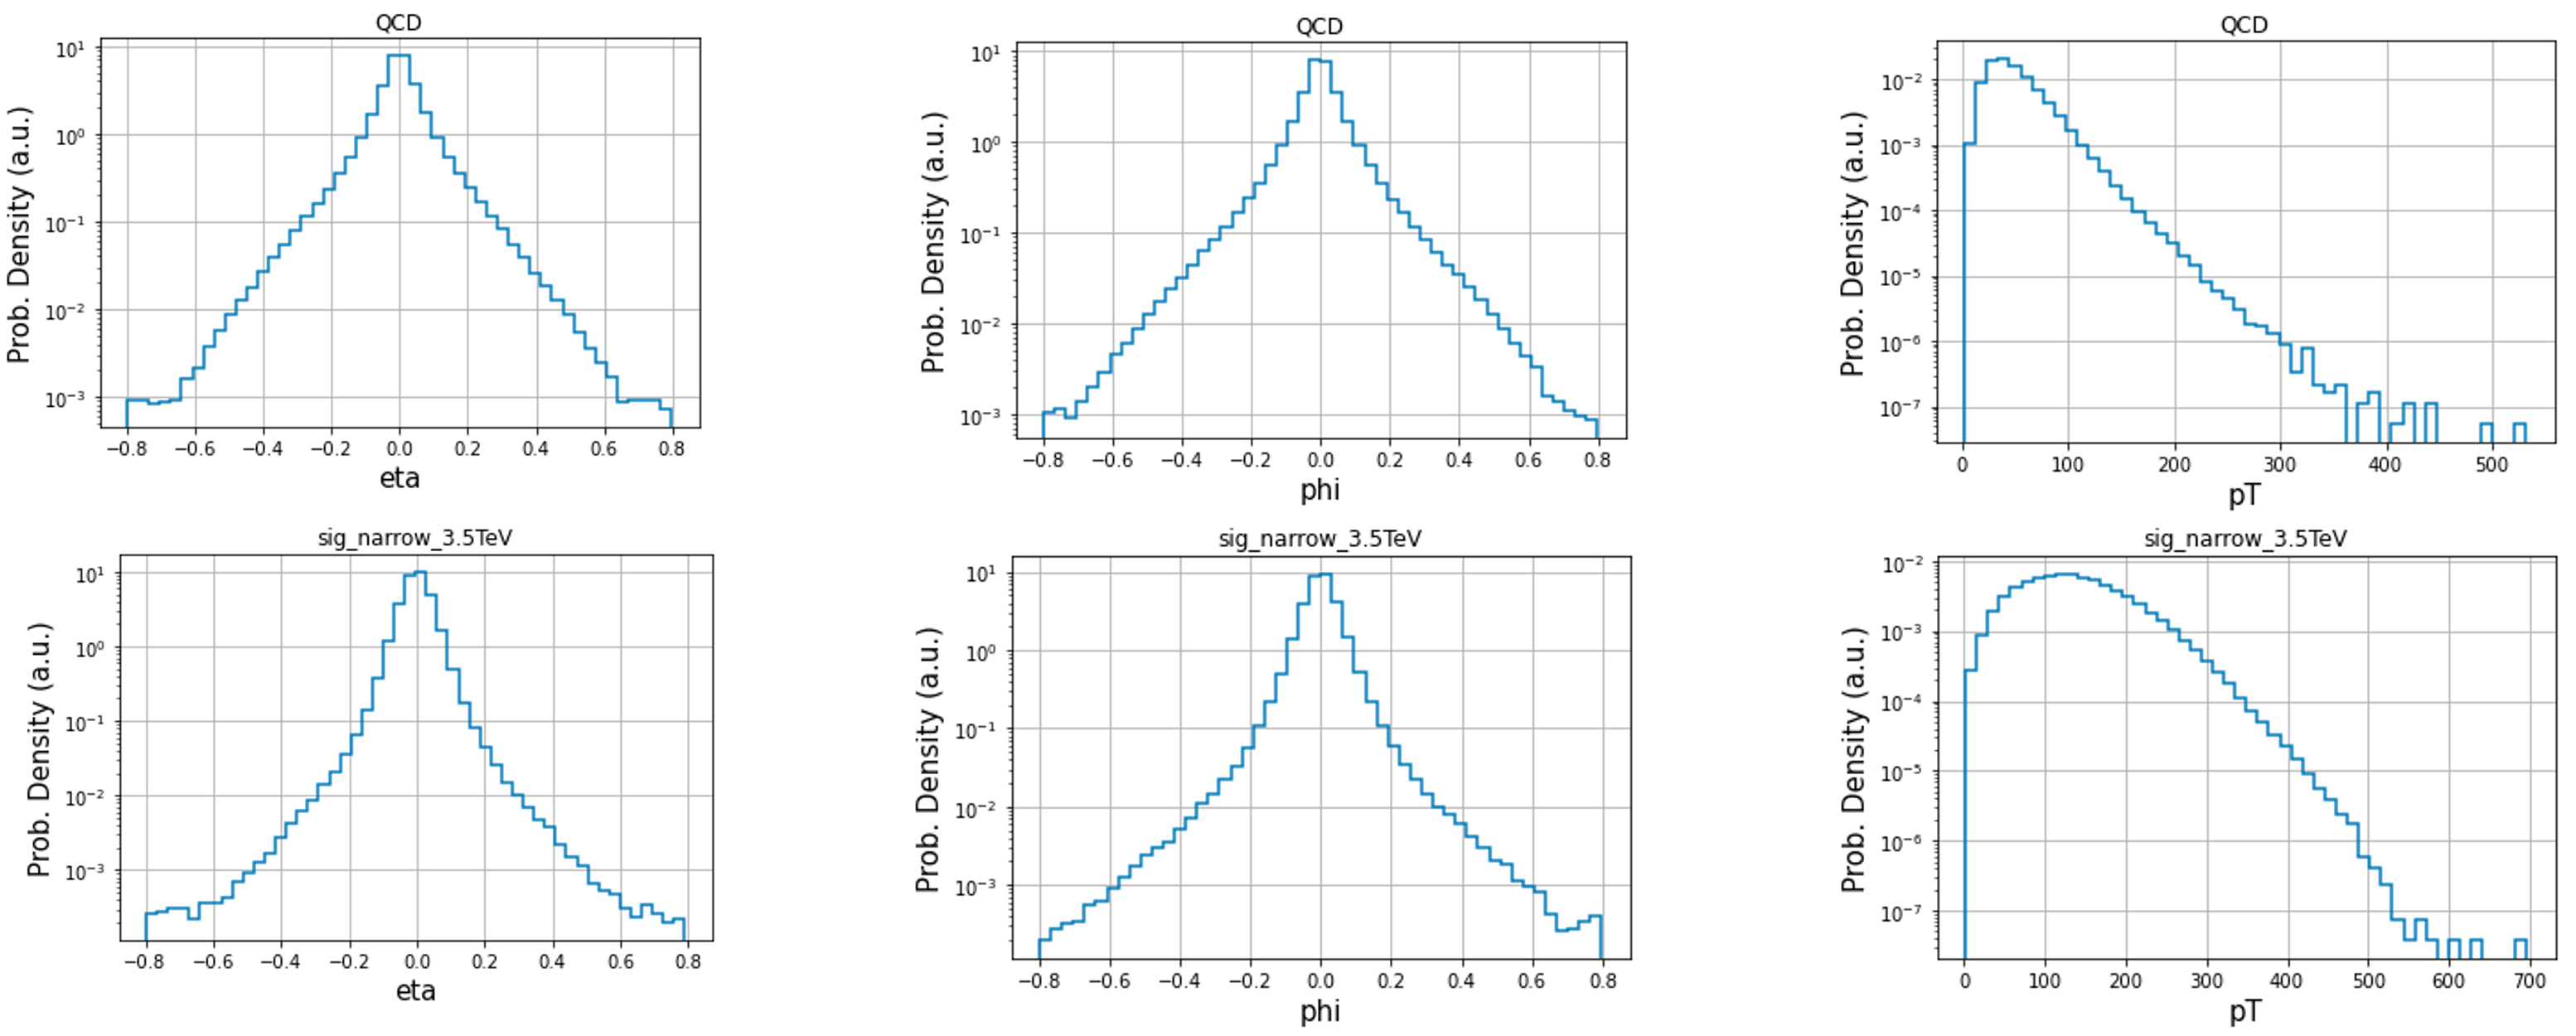
\includegraphics[width=\textwidth]{data.png}
			\caption{Plots of the datasets that are used as inputs to the models, QCD is the background data that's used for training, and "sig\_narrow\_3.5TeV" is one of the 4 signal datasets. These values are considered raw.}
			\label{fig:data}
		\end{minipage}
	\end{figure}
	
	\section{Autoencoders}
	\label{section:autoencoders}

		For the model architectures, only non-variational autoencoders were explored; those being the CNN and GarNet-Dense autoencoders. During training, both models were trained for 30 epochs (both models plateau around the 10 epoch mark) with a batch size of 1024. The models were compiled with the Adam optimisation algorithm \cite{adam} in order to minimise the cross-entropy error function over the entire training set, and the learning rate ($\alpha$) was set to $10^{-3}$. Both models also use the same loss function, mean squared error loss function (MSE), and it is described by Equation \ref{mse}.

		\begin{equation}\label{mse}
			MSE =  \frac{1}{n} \sum_{i=0}^{n} (Y_i - \hat{Y_i})^2
		\end{equation}

		Where $n$ is the number of predictions, $Y_i$ is the predicted value, and $\hat{Y_i}$ is the input value.

		\subsection{Convolutional Neural Network}

			Although the background dataset used for training is not image data, the tabular data has been treated as a 2D image in order for us to use the CNN architecture. As shown in Figure \ref{fig:cnn-encoder}, the encoder CNN architecture has 2 2D Convolutional layers (Conv2D) with ReLU activation to avoid the vanishing gradients problem, 2 2D Average Pooling layers, a Dense layer, and a Flatten layer. The input here is the dataset with a dimension of $16 \times 3 \times 1$ for each of the over three million jet constituents. The dataset has been scaled up to three dimensions in order to be able to use the 2D functions provided by Keras. The first Conv2D layer uses 16 $3 \times 3$ kernels, while the second has 32 $3 \times 1$ kernels. Both Average Pooling layers use a pool size of $3 \times 1$. The Dense, and final, layer uses 8 units which is the dimensionality of the latent space, and unlike the convolutional layers, it is not activated.

			As for the decoder - which is shown in Figure \ref{fig:cnn-decoder} - it uses 3 Conv2D layers with ReLU activation just like the encoder, 3 Up Sampling 3D layers, a reshape layer, and a dense layer. The input for the decoder is the output of the encoder, which is to say the input is the latent space. The first two Conv2D layers use 32 $3 \times 1$ kernels and 16 $3 \times 1$ kernels respectively, whereas the last Conv2D uses a single $3 \times 3$ kernel. Here the Dense layer uses 32 units. The reshape layer is needed to increase the number of dimensions of the "image" from 2D to 3D. Up Sampling can be thought of as the opposite of average pooling as the decoder is transforming the latent space back into the dimensionality of the input dataset.

			\begin{figure}[H]
				\centering
					\begin{minipage}[c]{0.45\linewidth}
						\centering
						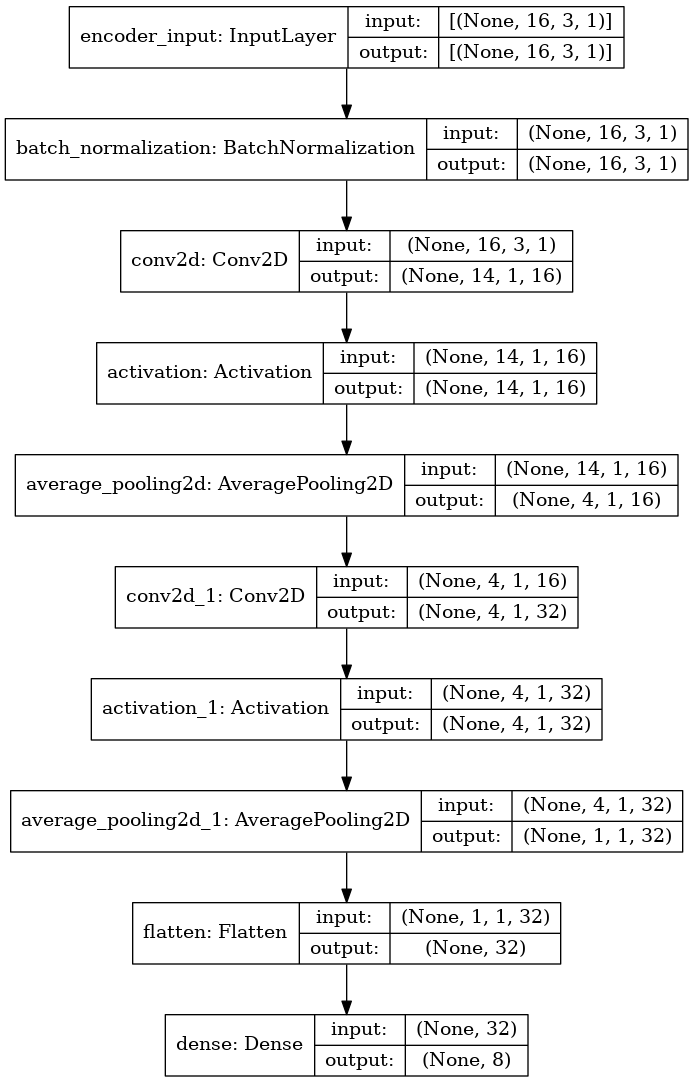
\includegraphics[width=0.8\textwidth]{encoder.png}
						\caption{CNN enocder, which is the first half of the CNN AE. Each rectangle represents a layer and the arrows incdicates the direction of model, from input (dataset) to output (latent space). Each layer also indicates its local input and output shapes. }
						\label{fig:cnn-encoder}
					\end{minipage}
				\hfill
					\begin{minipage}[c]{0.45\linewidth}
						\centering
						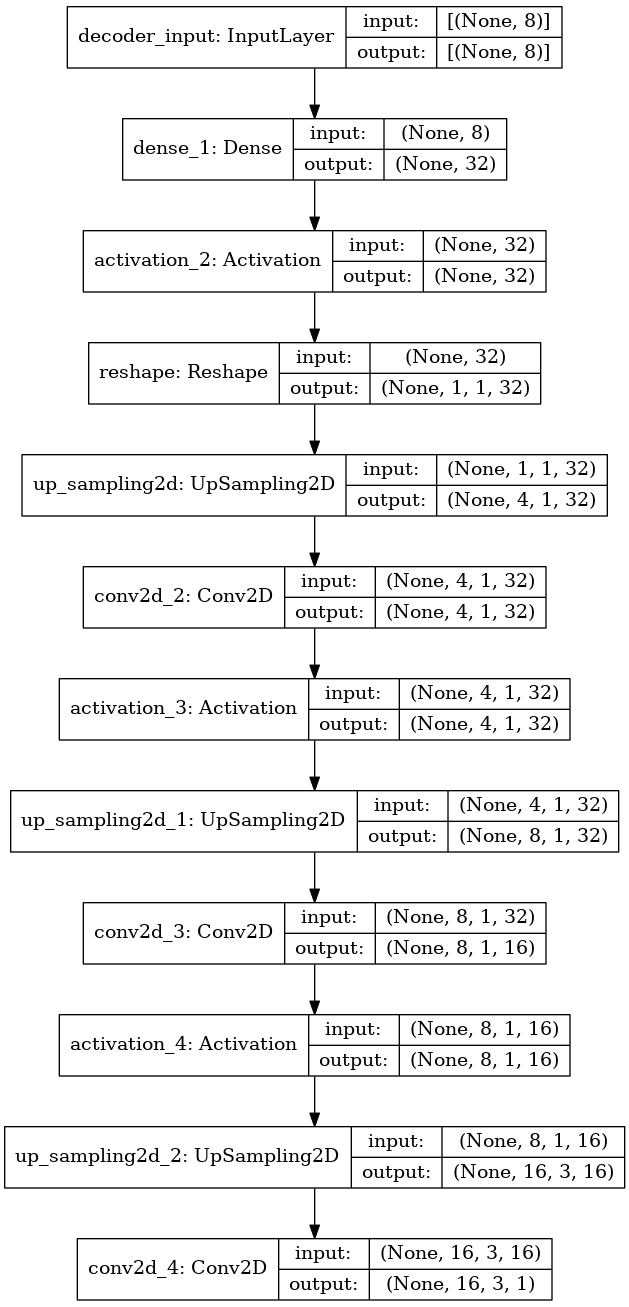
\includegraphics[width=0.8\textwidth]{decoder.png}
						\caption{CNN decoder, which is the second half of the CNN AE. The schema for this has been described in Figure \ref{fig:cnn-encoder}.}
						\label{fig:cnn-decoder}
					\end{minipage}
			\end{figure}

			In total, this results in 6988 trainable parameters with only 2 non-trainable parameters. 5040 of which come from the decoder, as the process of decoding is significantly harder than encoding data and was where the bulk of the work was concentrated upon. 

			The quantised and pruned version of this model follows the same architecture structure but with fewer bits per weight and fewer overall weights. This model was tested from 2 bits widths to 16 in increments of 2, and the sparsity for pruning was set to 50\%. QKeras \cite{qkeras} was used to perform the quantisation. 

		\subsection{GarNet-Dense}

			This model is not a full graph autoencoder, instead only the encoder uses a graph architecture (more specifically a single GarNet layer) and the decoder uses a DNN architecture. As shown by Figure \ref{fig:garnet-model}, the GarNet-Dense autoencoder takes in two inputs, the data which is $16 \times 3$ and an adjacency matrix that has a dimension of one. The model encodes the input down to the latent space (with a dimension of 8) using a single GarNet layer \cite{garnet}, and then uses 4 Dense layers, a reshape layer, and an Up Sampling 2D layer in order to produce the reconstructed features. The GarNet layer used here has 32 propagators, 8 filters, 32 aggregators, and it uses the ReLU activation function. In the decoder, all Dense layers but the last use 32 units and the sigmoid function for activation, the last Dense layer uses 16 units and the softmax function for activation. The reshape layer is needed to increase the number of dimensions so that the Up Sampling 2D layer can be used to match the input to this autoencoder. 
				
			\begin{figure}[H]
				\centering
				\begin{minipage}[b]{\linewidth}
					\centering
					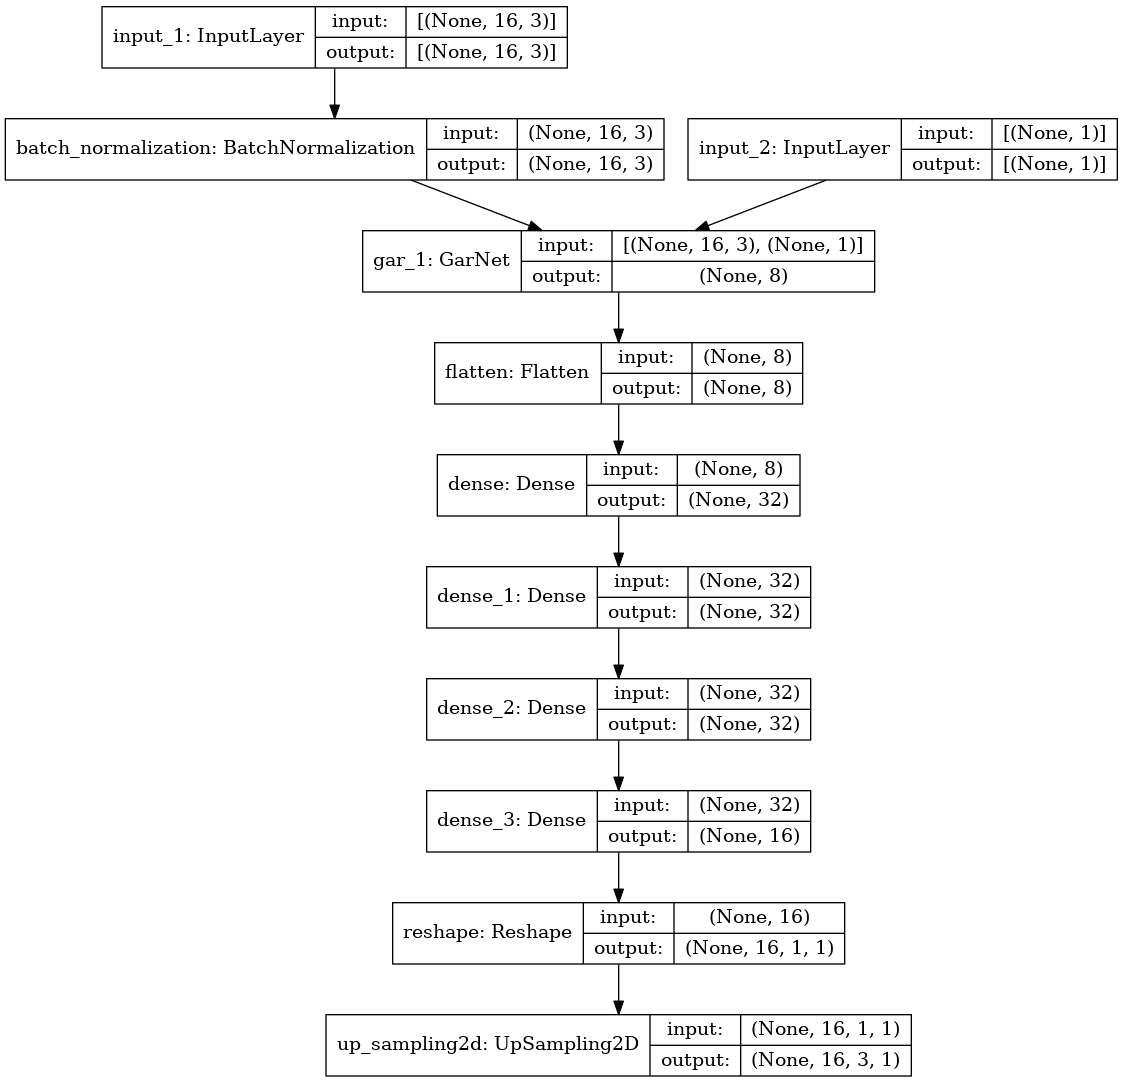
\includegraphics[width=0.7\textwidth]{model.png}
					\caption{The entire GarNet-Dense AE layout. The schema for this has been described in Figure \ref{fig:cnn-encoder}.}
					\label{fig:garnet-model}
				\end{minipage}
			\end{figure}





	
	\section{Results}
	\label{section:results}

		In this chapter, the results of the CNN and GarNet-Dense AEs are discussed, which includes the training that's used to show how well the models fit the data, the reconstructed features show how models are able to encode and then decode the data, loss distributions which are used to inspect how the model was able to separate the background from the signals, and finally the Receiver Operating Characteristic (ROC) curves and AUC (Aread Under the ROC Curve) scores which are used to quantify how well the models perform given the signal data.

		\subsection{Training}
			
			The plots for the distribution of the MSE loss as a function of the number of epochs (training and validation history) for the CNN AE are shown in Figure \ref{fig:cnn-training}, while the training and validation history for the quantised (8-bits) and pruned CNN AE model is shown in Figure \ref{fig:cnn-compressed-training}. Since all models show a significant reduction in loss, they are not underfitting. However, The normalised CNN AE model plateaus much quicker than the rest suggesting that it does not fit as well as the others. Since both the training and validation history are close to each other, the models do not overfit the data.

			\begin{figure}[H]
				\centering
				\begin{minipage}[c]{0.45\linewidth}
					\centering
					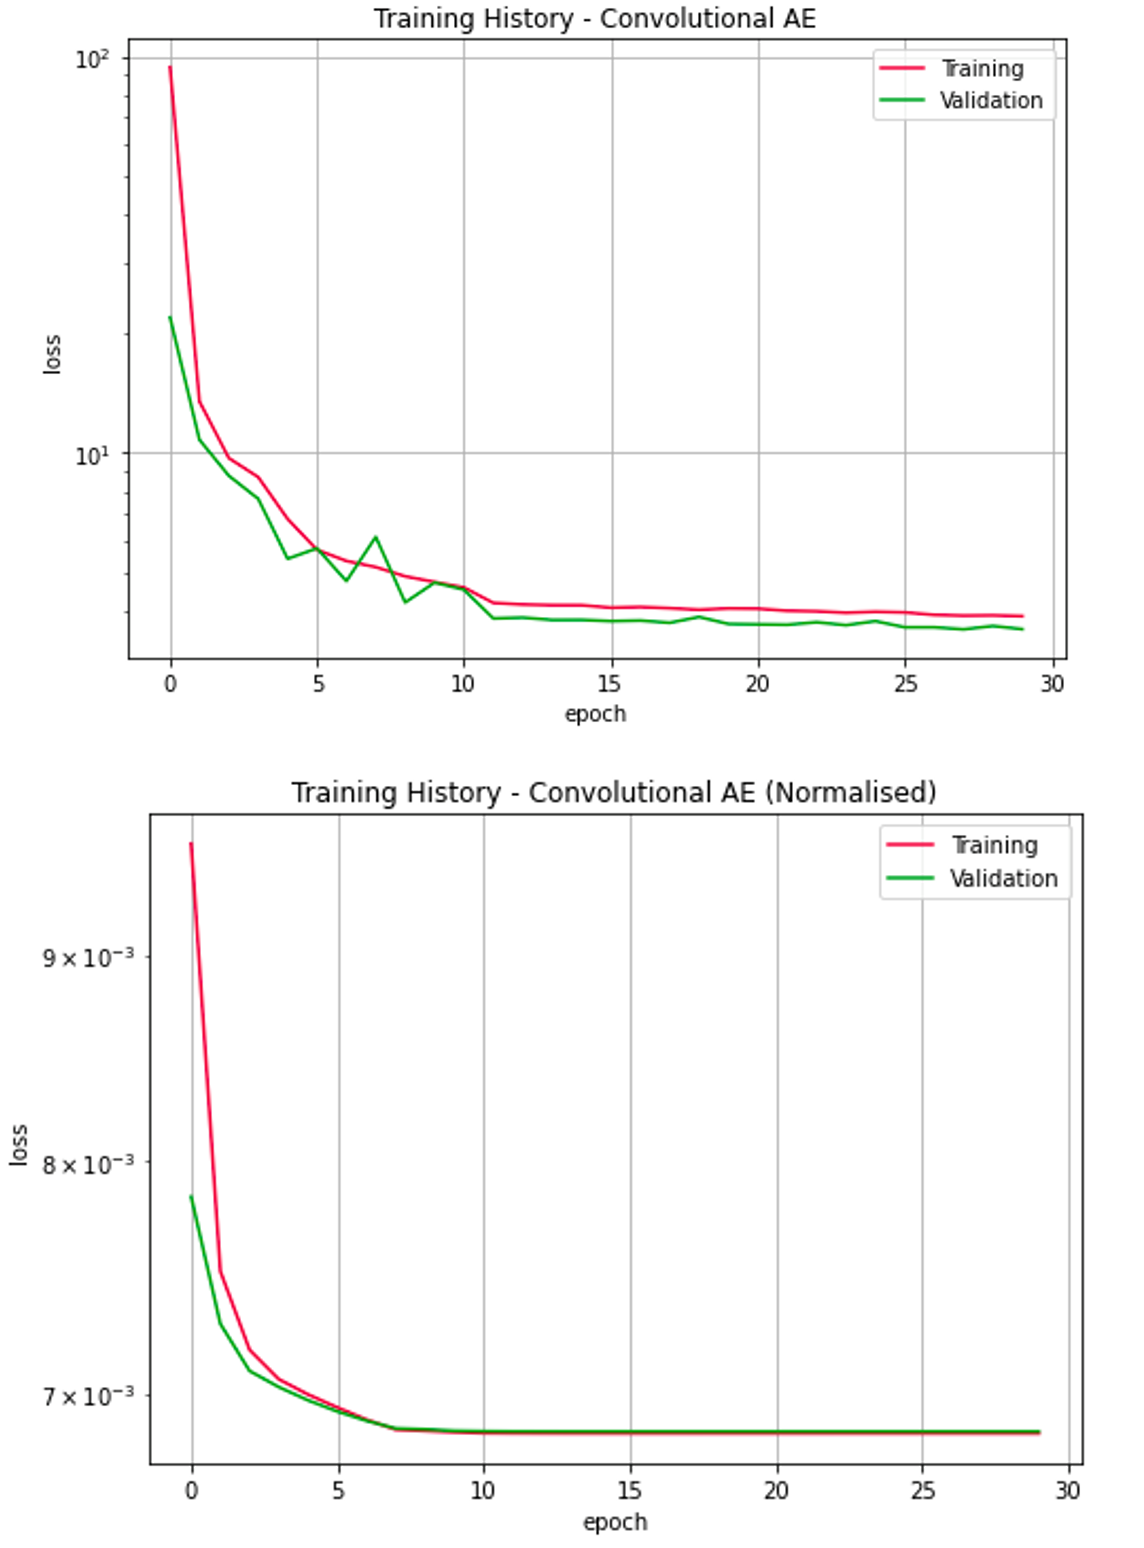
\includegraphics[width=\textwidth]{cnn-training.png}
					\caption{The top plot represents the regular CNN AE's training and validation history, while the bottom is the training and validation history for the CNN AE with the normalised version of the dataset as the training and validation data.}
					\label{fig:cnn-training}
				\end{minipage}
				\hfill
				\begin{minipage}[c]{0.45\linewidth}
					\centering
					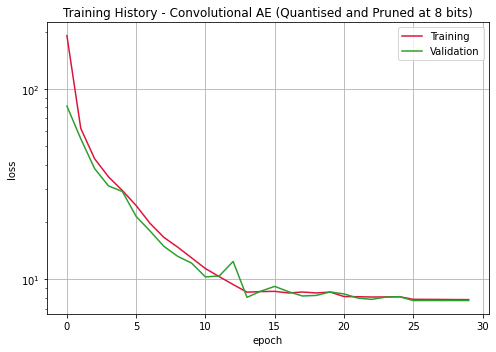
\includegraphics[width=\textwidth]{cnn-compressed-training.png}
					\caption{The training and validation history for the quantised and pruned CNN AE model.}
					\label{fig:cnn-compressed-training}
				\end{minipage}
			\end{figure}

			The training and validation history for GarNet-Dense can be seen in Figure \ref{fig:garnet-training}, where the model virtually does not train given the raw dataset as the input; the model is severely underfitting the data. When the dataset used for training is normalised, however, the CNN AE model is able to train somewhat, given the small reduction in loss the training for GarNet is not ideal and it is still underfitting the data but to a lesser extent. 

			\begin{figure}[H]
				\centering
				\begin{minipage}[b]{\linewidth}
					\centering
					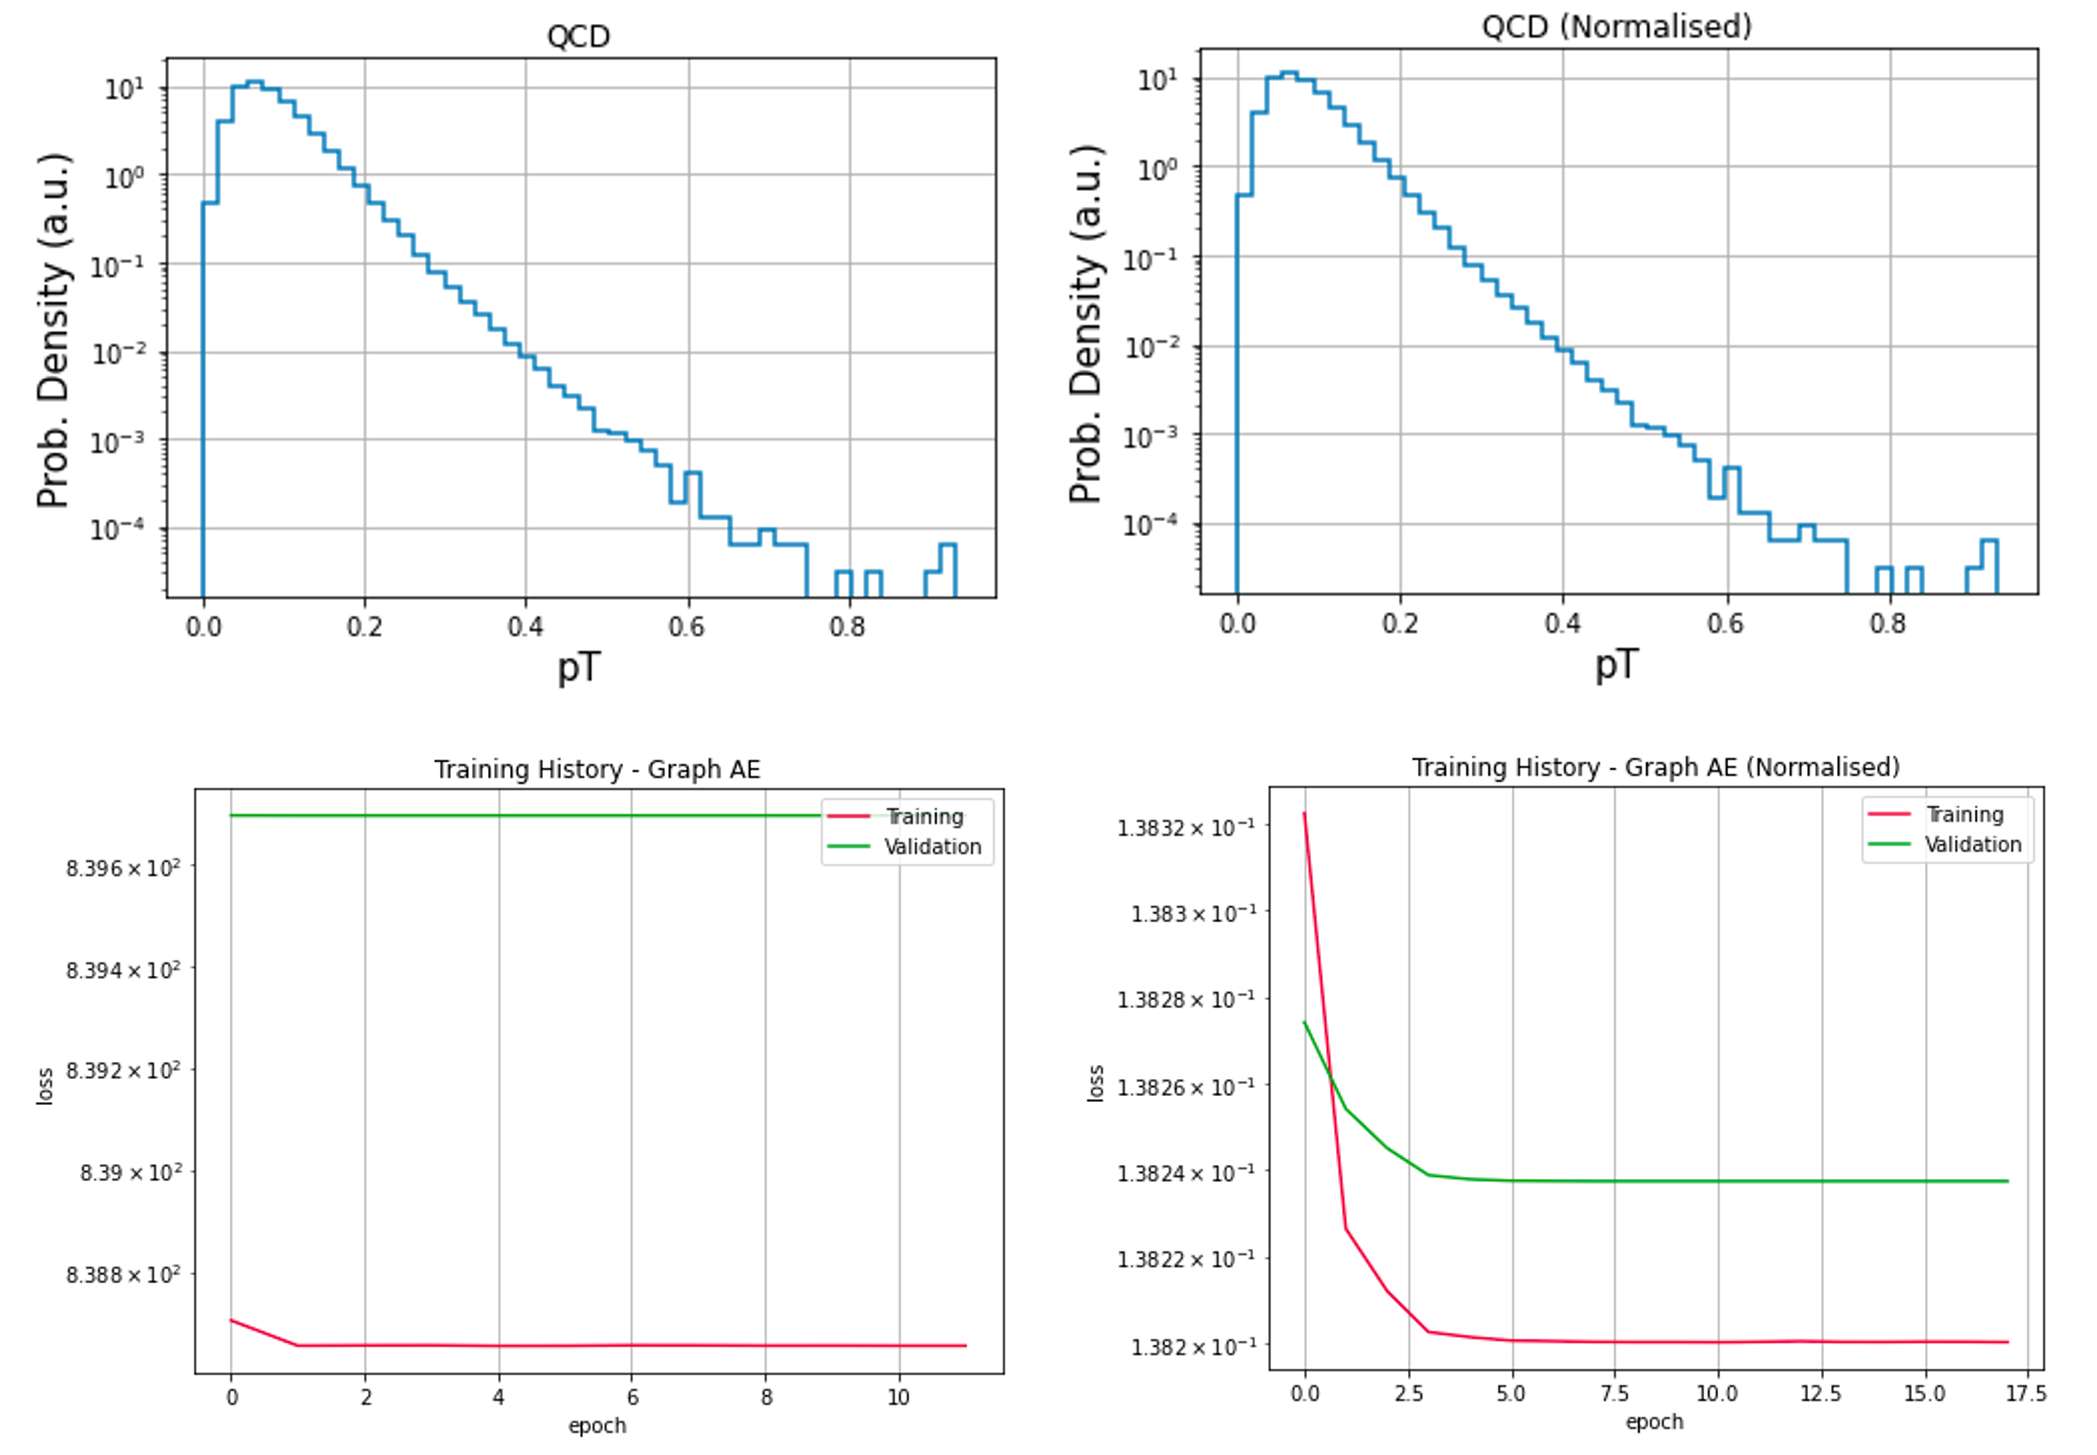
\includegraphics[width=0.8\textwidth]{garnet-training.png}
					\caption{The dataset normalisation and training and validation history for GarNet-Dense, while $p_T$ was the only feature shown here, the other 2 features were also normalised.}
					\label{fig:garnet-training}
				\end{minipage}
			\end{figure}



		\subsection{Reconstructed Features}

			The CNN AE is able to reconstruct the features well (shown in Figure \ref{fig:cnn-reconstructed}), especially the $p_T$ feature where, for the background dataset, it is able to almost perfectly match it; it only falls short towards the higher $p_T$ values. As expected, the model performs worse for the signal data, where the reconstructed $\phi$ and $\eta$ features are much narrower when compared to the reconstruction of those features for the background data. Due to the higher values of $p_T$, the model is biasing towards it, which results in an inferior reconstruction for the other features.

    		\begin{figure}[H]
				\centering
				\begin{minipage}[b]{\linewidth}
					\centering
					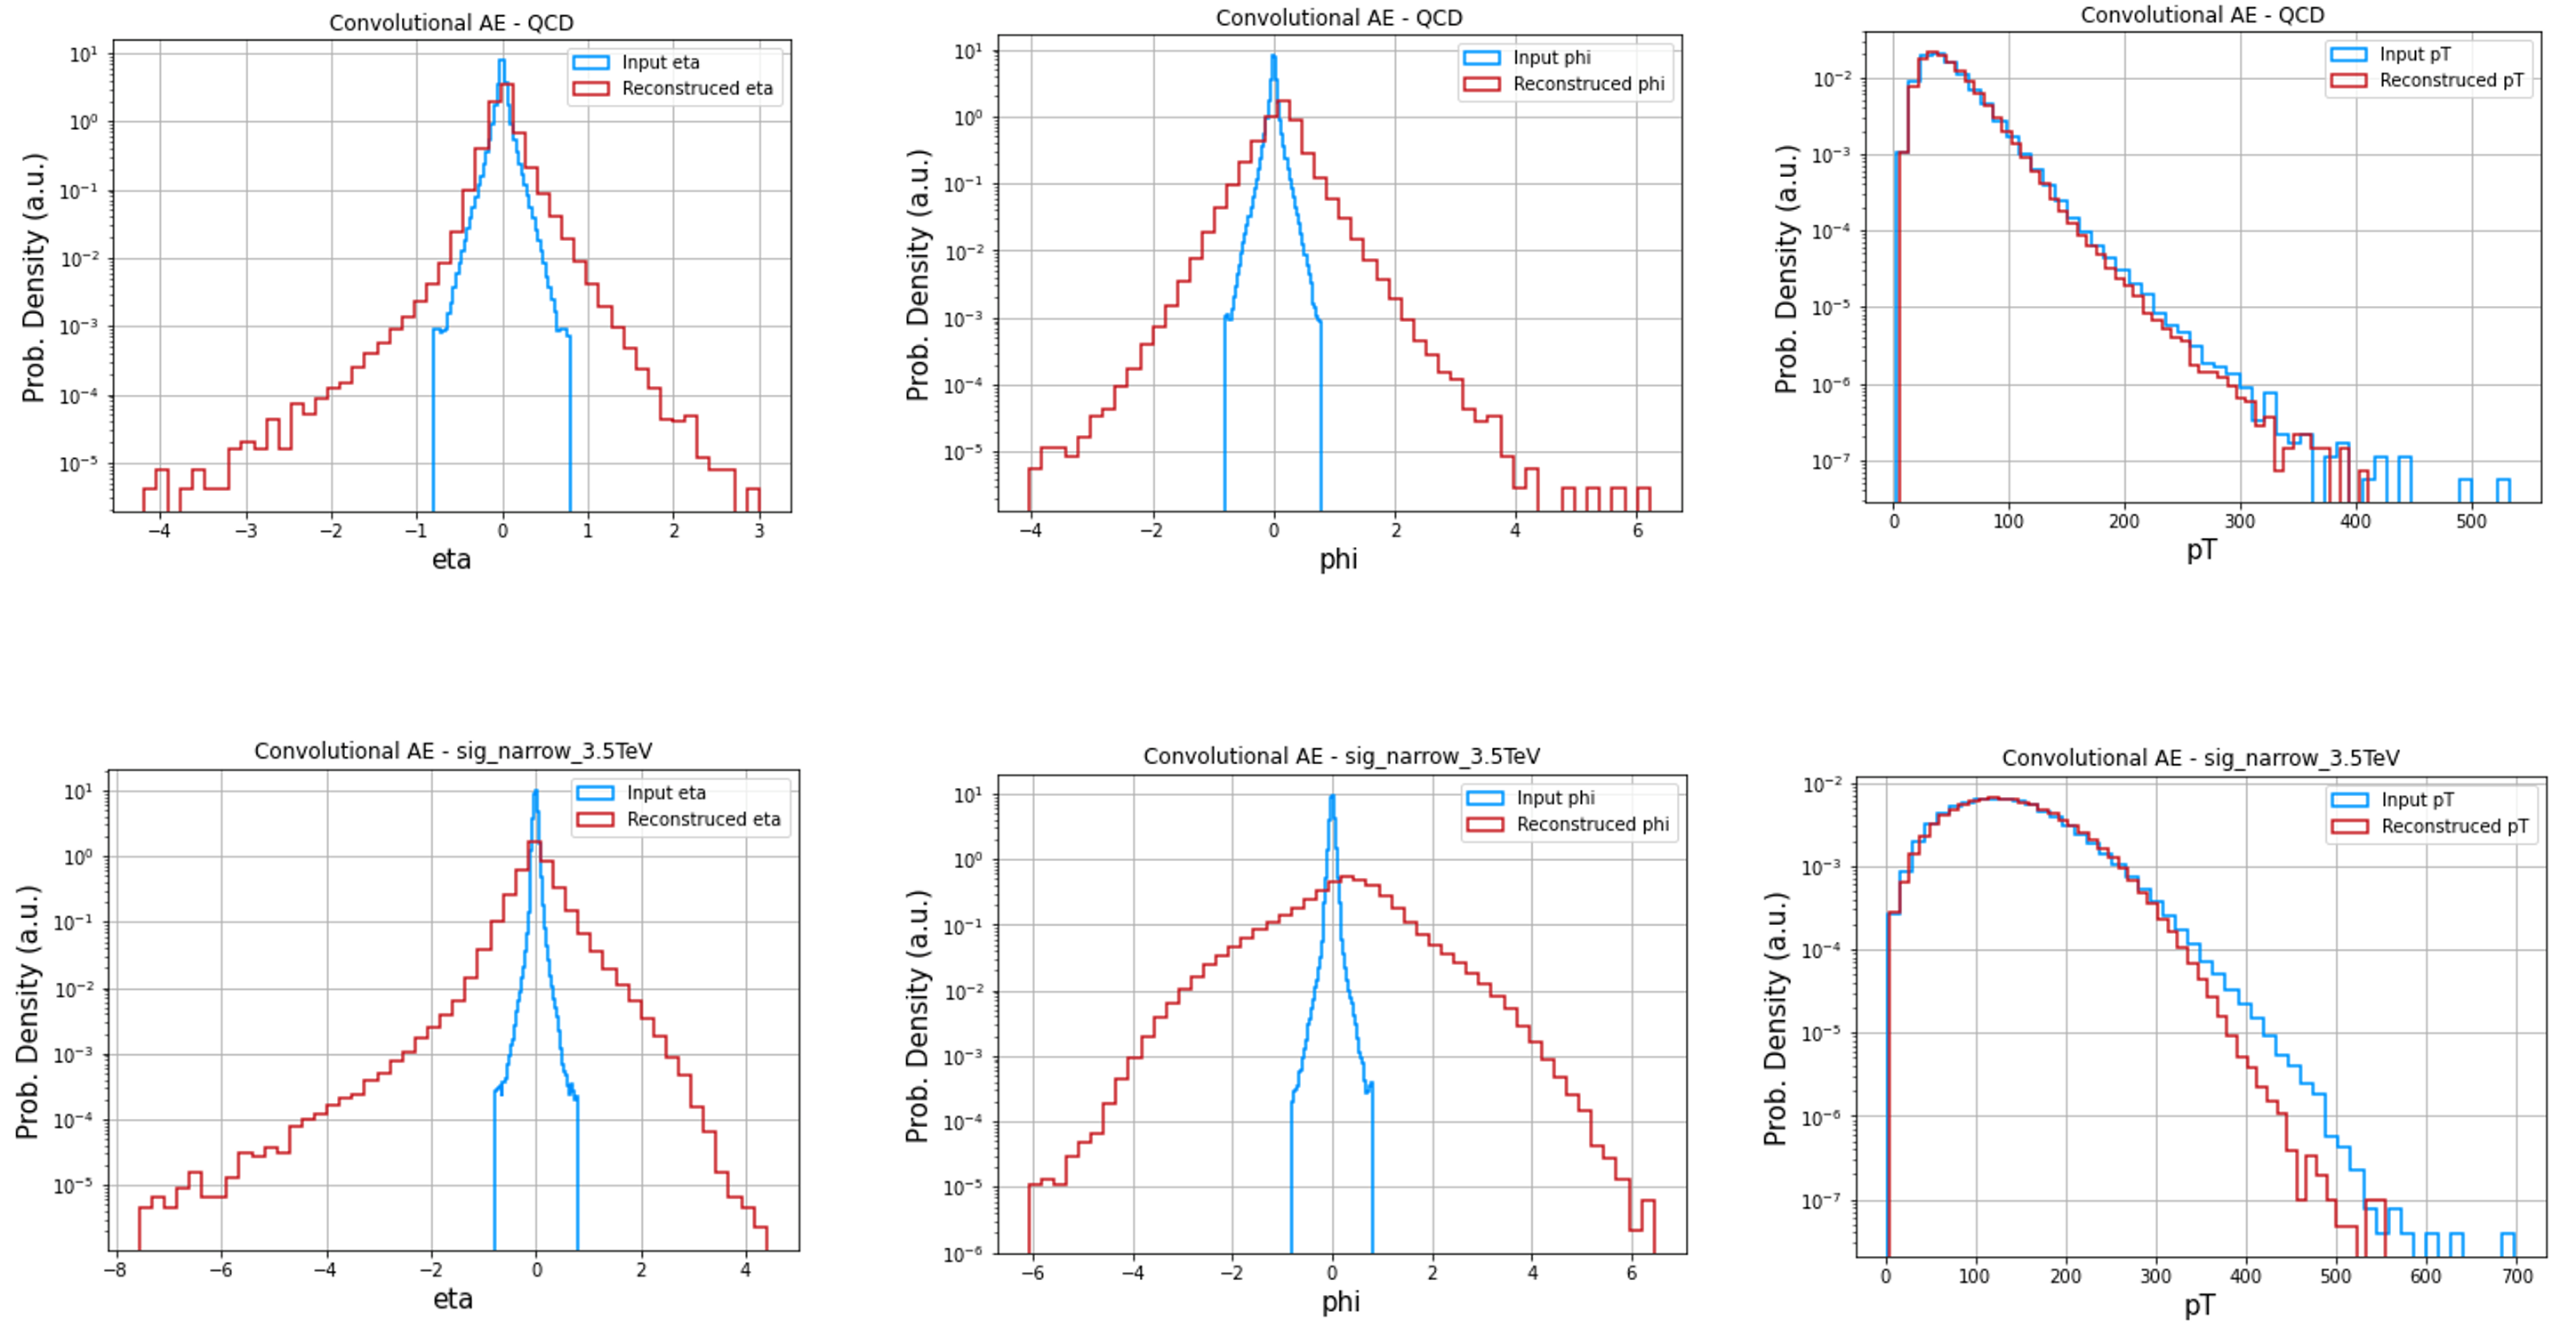
\includegraphics[width=\textwidth]{cnn.png}
					\caption{The reconstructed features for background (QCD) and the narrow $3.5 TeV$ signal datasets produced from the regular CNN AE. Only one signal dataset was shown here for the sake of simplicity.}
					\label{fig:cnn-reconstructed}
				\end{minipage}
			\end{figure}

			In order to combat the issue of the model biasing towards $p_T$, all features for both the background and signal data were normalised using the MinMax algorithm. The result of which is shown in Figure \ref{fig:cnn-recontructed-norm}. As expected the model no longer biases as much towards $p_T$ and the reconstruction for the other features improves - at the cost of worse $p_T$ reconstruction. However, what was not expected was the minimal difference between the background and signal data for the $\phi$ and $\eta$ features. They produce a similar reconstruction to their respective input data, where a worse reconstruction was expected for the signal data when compared to the background data. 

    		\begin{figure}[H]
				\centering
				\begin{minipage}[b]{\linewidth}
					\centering
					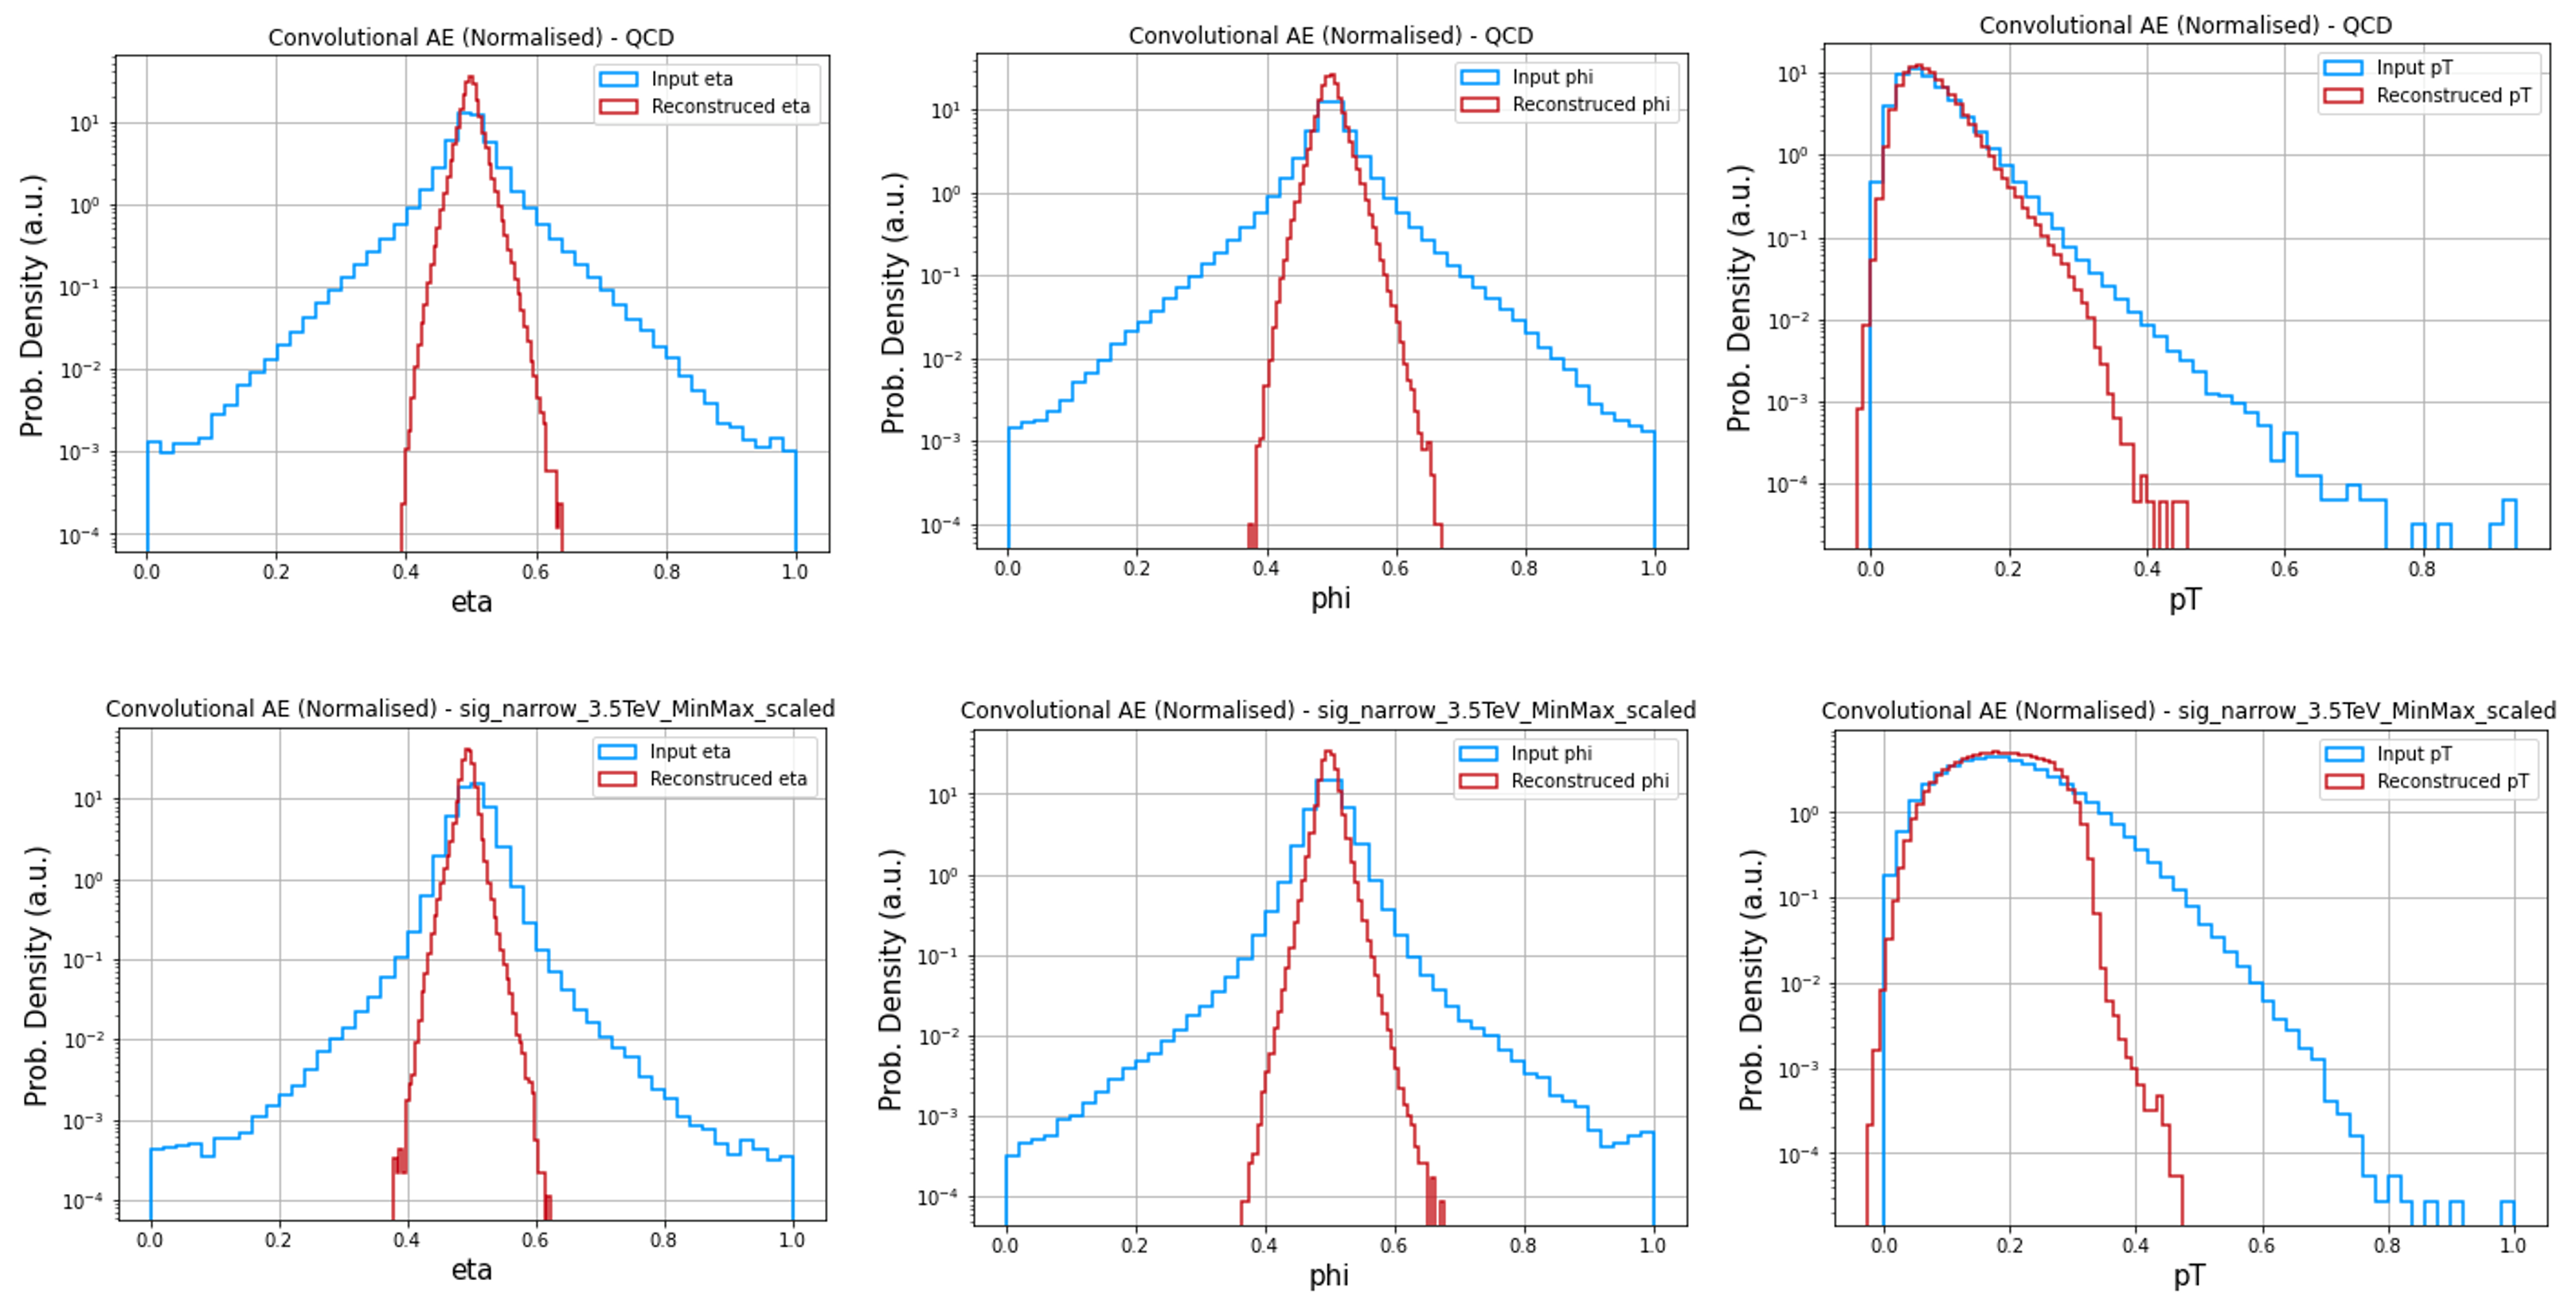
\includegraphics[width=\textwidth]{cnn-norm.png}
					\caption{The reconstructed features for background (QCD) and the narrow $3.5 TeV$ signal datasets produced from the normalised datasets and CNN AE, which is why the x-axis is different when compared to the regular CNN AE reconstructed features (Figure \ref{fig:cnn-reconstructed}).}
					\label{fig:cnn-recontructed-norm}
				\end{minipage}
			\end{figure}

			Shown in Figure \ref{fig:garnet-reconstruction} is the reconstructed features produced from the GarNet-Dense AE. The results are not favourable, but not unexpected, as we saw poor data fitting in the training plots for this model (Figure \ref{fig:garnet-training}). Had the model trained even somewhat properly, the reconstructed features would have centered around the 0 value for each respective feature, instead we see a skewed reconstruction that is heavily biased towards lower values. There is very little to separate the background and the signal reconstruction, which suggests this model will perform poorly when it comes to loss and the AUC metric. 

    		\begin{figure}[H]
				\centering
				\begin{minipage}[b]{\linewidth}
					\centering
					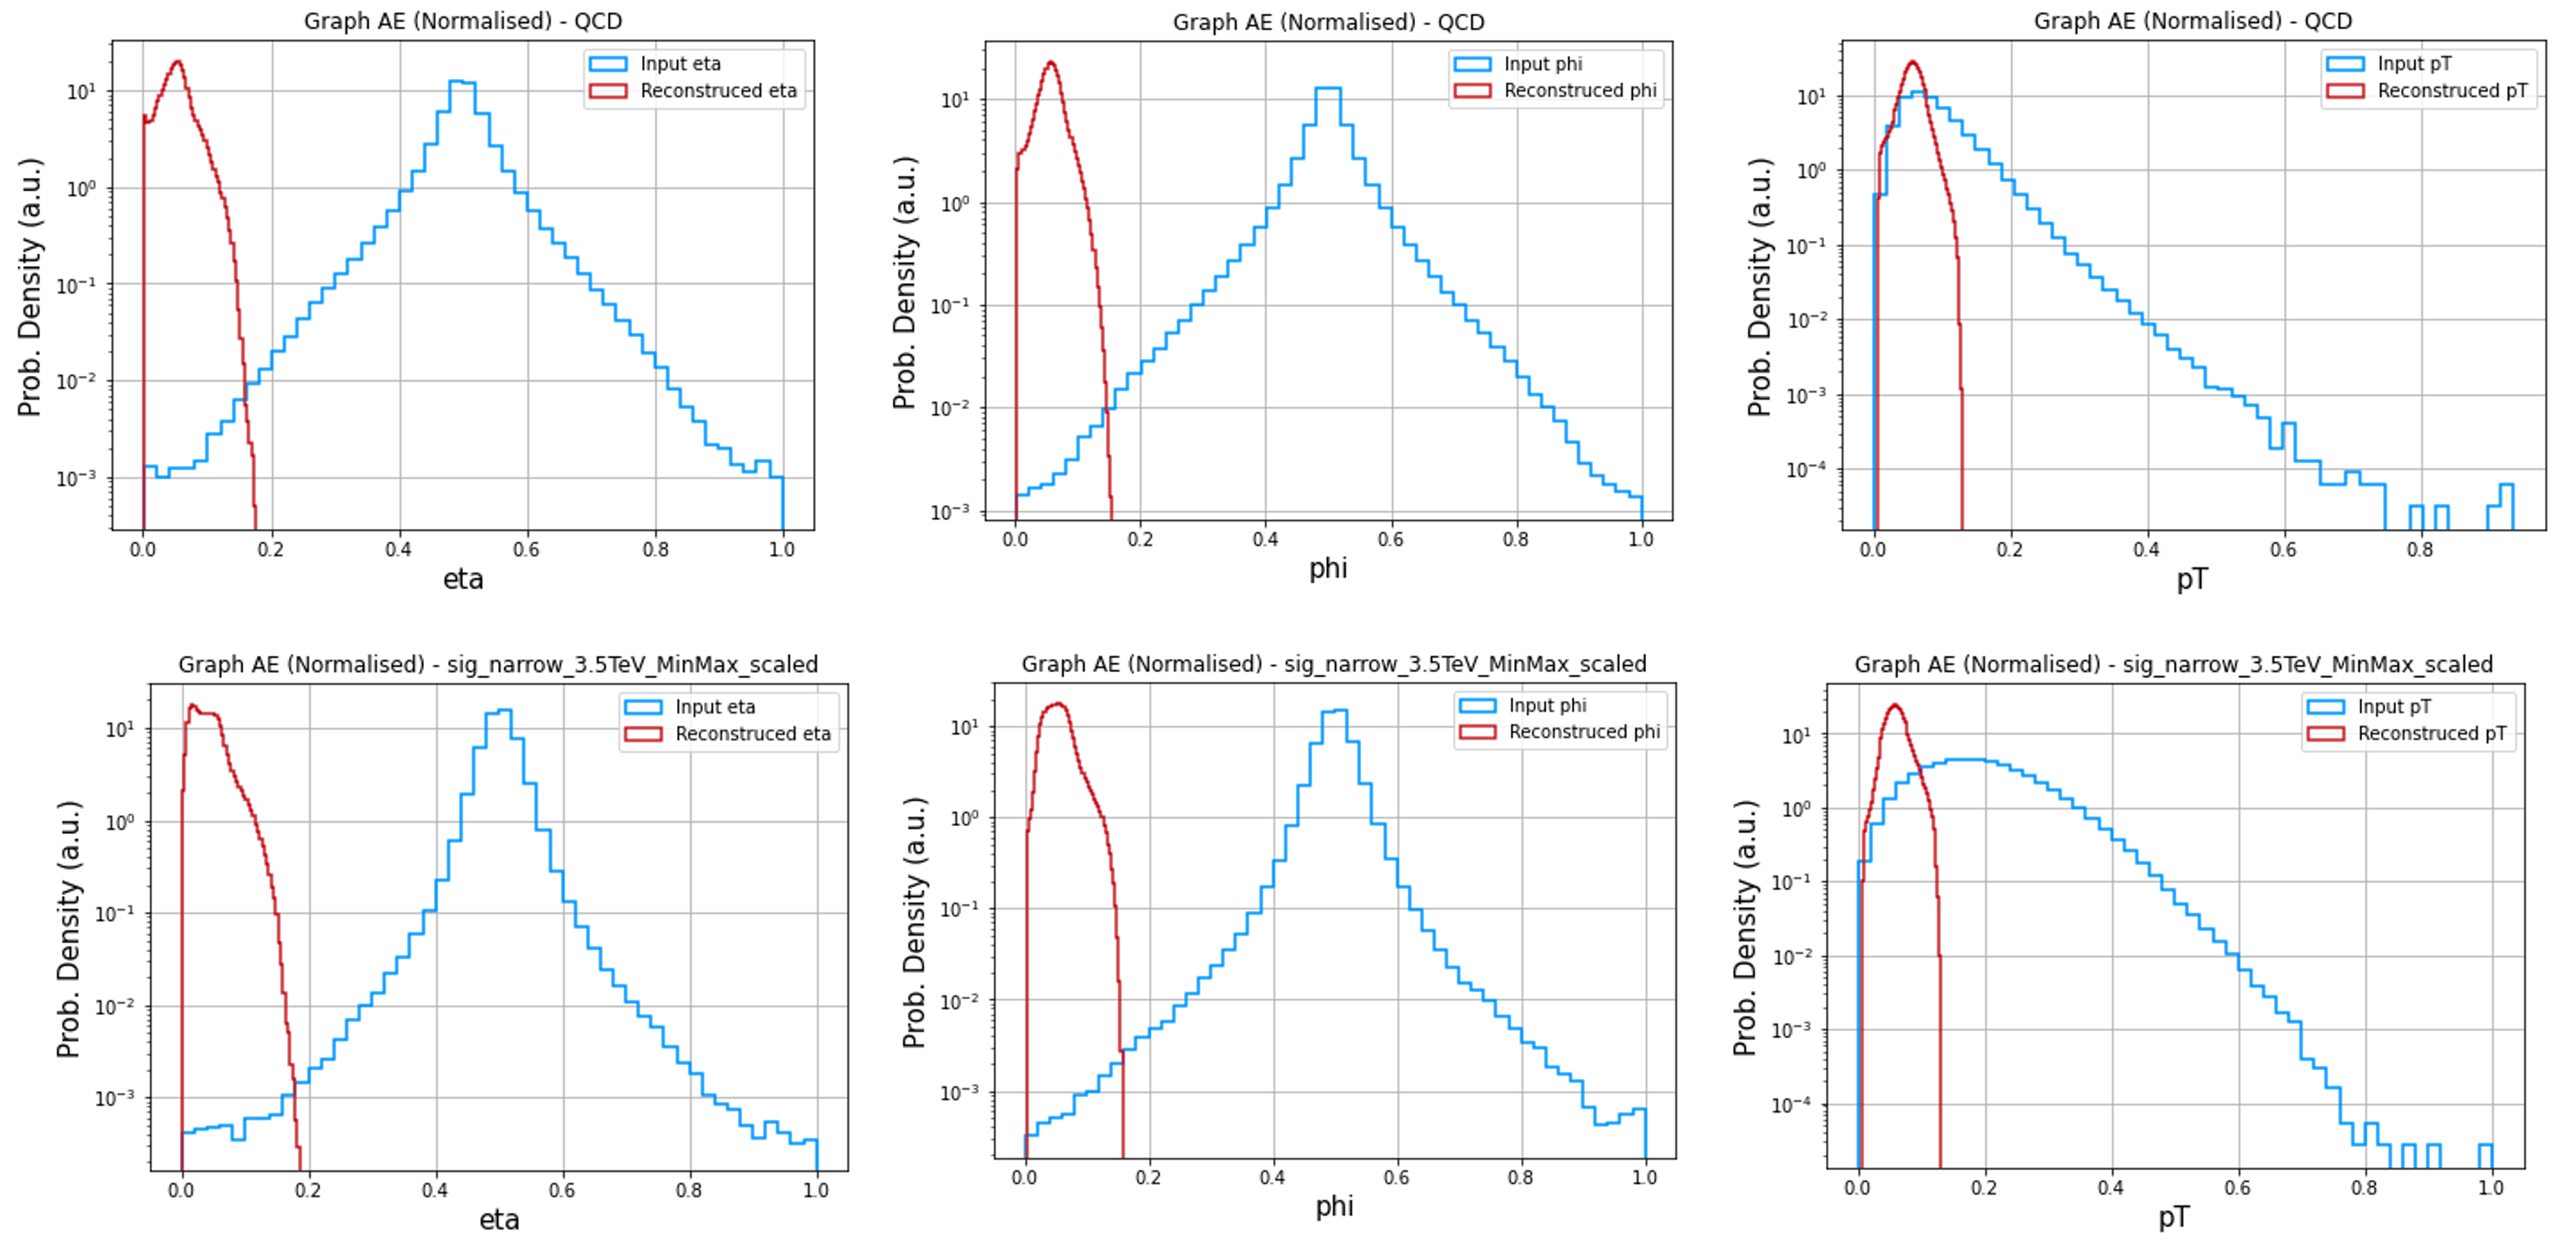
\includegraphics[width=\textwidth]{garnet.png}
					\caption{The reconstructed features for background (QCD) and the narrow $3.5 TeV$ signal datasets produced from the GarNet-Dense AE model with the normalised datasets.}
					\label{fig:garnet-reconstruction}
				\end{minipage}
			\end{figure}

		\subsection{Loss Distributions}

			The loss distribution for the CNN AE (both using normalised and raw data) is shown in Figure \ref{fig:cnn-loss}, and as was seen in the reconstruction of the features of both of these AEs, when the CNN AE is trained on the raw data it is able to separate the background and signal data much better than the normalised version; especially for the higher valued $3.5  TeV$ signal datasets. This shows that normalising the data, while it removes the heavy bias towards $p_T$, produces worse results. 

			The quantised and pruned CNN AE model (shown in Figure \ref{fig:cnn-compressed-loss}) also does a good job of separating the background from the signal data, although it produces higher AE loss values due to the weights having a lower number of bits to represent the data, which is expected. Again, just like the unquantised and unpruned model, the higher valued $3.5  TeV$ signal datasets show the greater amount of separation from the background. 

			\begin{figure}[H]
				\centering
					\begin{minipage}[c]{0.45\linewidth}
						\centering
						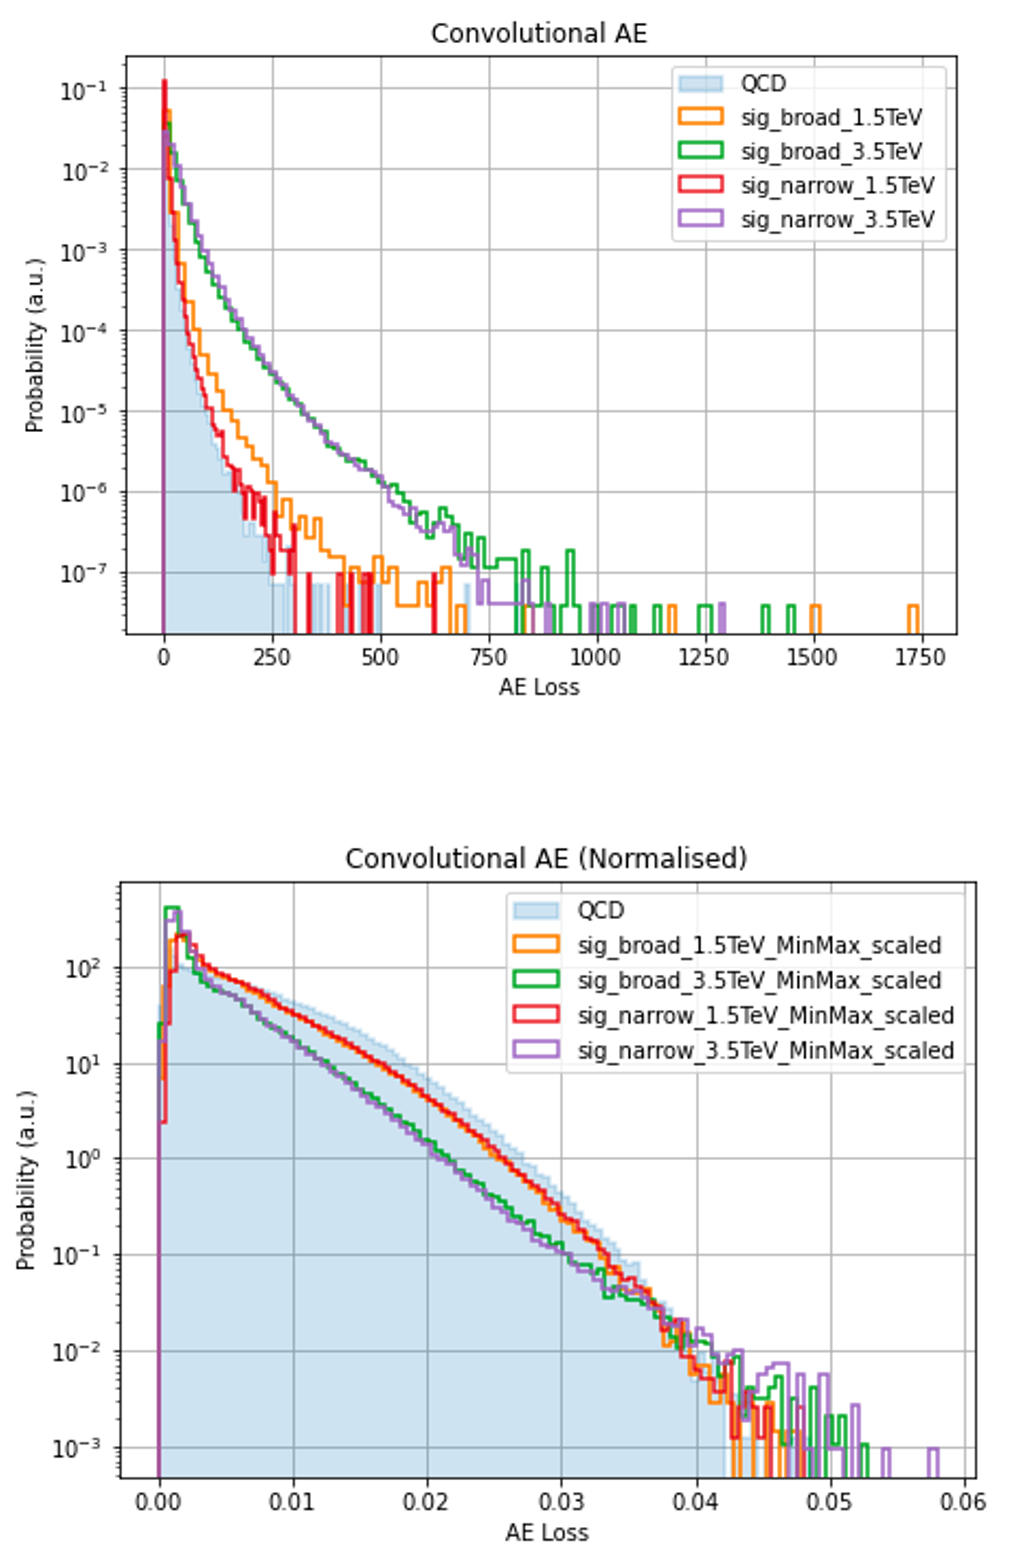
\includegraphics[width=\textwidth]{cnn-loss.png}
						\caption{The regular CNN AE loss distribution (top) and the normalsed dataset CNN AE loss distribution (bottom). Both show the losses for background (QCD) and the signals.}
						\label{fig:cnn-loss}
					\end{minipage}
					\hfill
					\begin{minipage}[c]{0.45\linewidth}
						\centering
						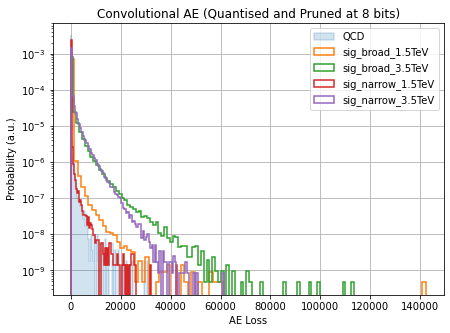
\includegraphics[width=\textwidth]{cnn-compressed-loss.png}
						\caption{The quantised and pruned CNN AE loss distribution. Showing the losses for background (QCD) and the signals.}
						\label{fig:cnn-compressed-loss}
					\end{minipage}
			\end{figure}

			Shown in Figure \ref{fig:garnet-loss} is the loss distribution for the GarNet-Dense AE, which faces a similar problem to the normalised CNN AE (Figure \ref{fig:cnn-loss}) in that it is not able to separate the background from the signal data well enough, which was also seen in GarNet-Dense's reconstruction plots (Figure \ref{fig:garnet-reconstruction}). This is due to the fact that the model did not really train and hence was not able to really learn the features of the data as expected.

			\begin{figure}[H]
				\centering
				\begin{minipage}[b]{\linewidth}
					\centering
					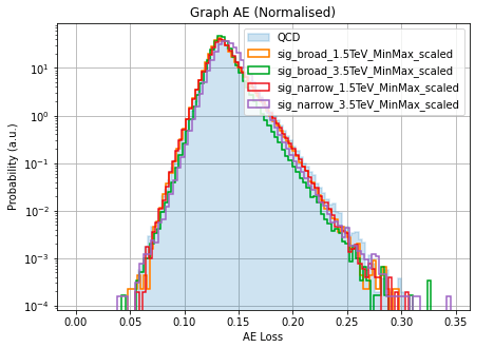
\includegraphics[width=0.5\textwidth]{garnet-loss.png}
					\small\caption{GarNet-Dense Loss distribution (normalised datasets).}
					\label{fig:garnet-loss}
				\end{minipage}
			\end{figure}

		\subsection{ROC Curves \& AUC Scores}

			Figure \ref{fig:cnn-roc} shows the ROC curves and AUC metric scores for the regular CNN AE with the unnormalised and normalised signal data, and as we saw with the loss plots, the higher valued signal data ($3.5  TeV$) produces the excellent AUC results - those being 88.3\% for the broad band and 92.3\% for the narrow band. The model performs well in terms of AUC with the lower valued signal data, showing that it is able to separate both sets of signal data well. However, the normalised version does not fare as well as it produces significantly worse AUC scores when compared. This is due to the model not being able to separate the background and signal data well, as was seen before with its loss and training plots (Figures \ref{fig:cnn-loss} and \ref{fig:cnn-training} respectively).

			Figure \ref{fig:cnn-compressed-roc} shows the same plot but with the quantised and pruned model, and this model is able to produce near-identical results to the unquantised and unpruned model as very little reduction, and in some cases, no reduction at all is seen in the AUC scores. Showing that even when compressed the model produces great results. Some of this difference between the compressed and uncompressed model can be attributed to training fluctuations, which could be mitigated by averaging over a set of trained models for each of the two model architectures. 


			\begin{figure}[H]
				\centering
					\begin{minipage}[c]{0.45\linewidth}
						\centering
						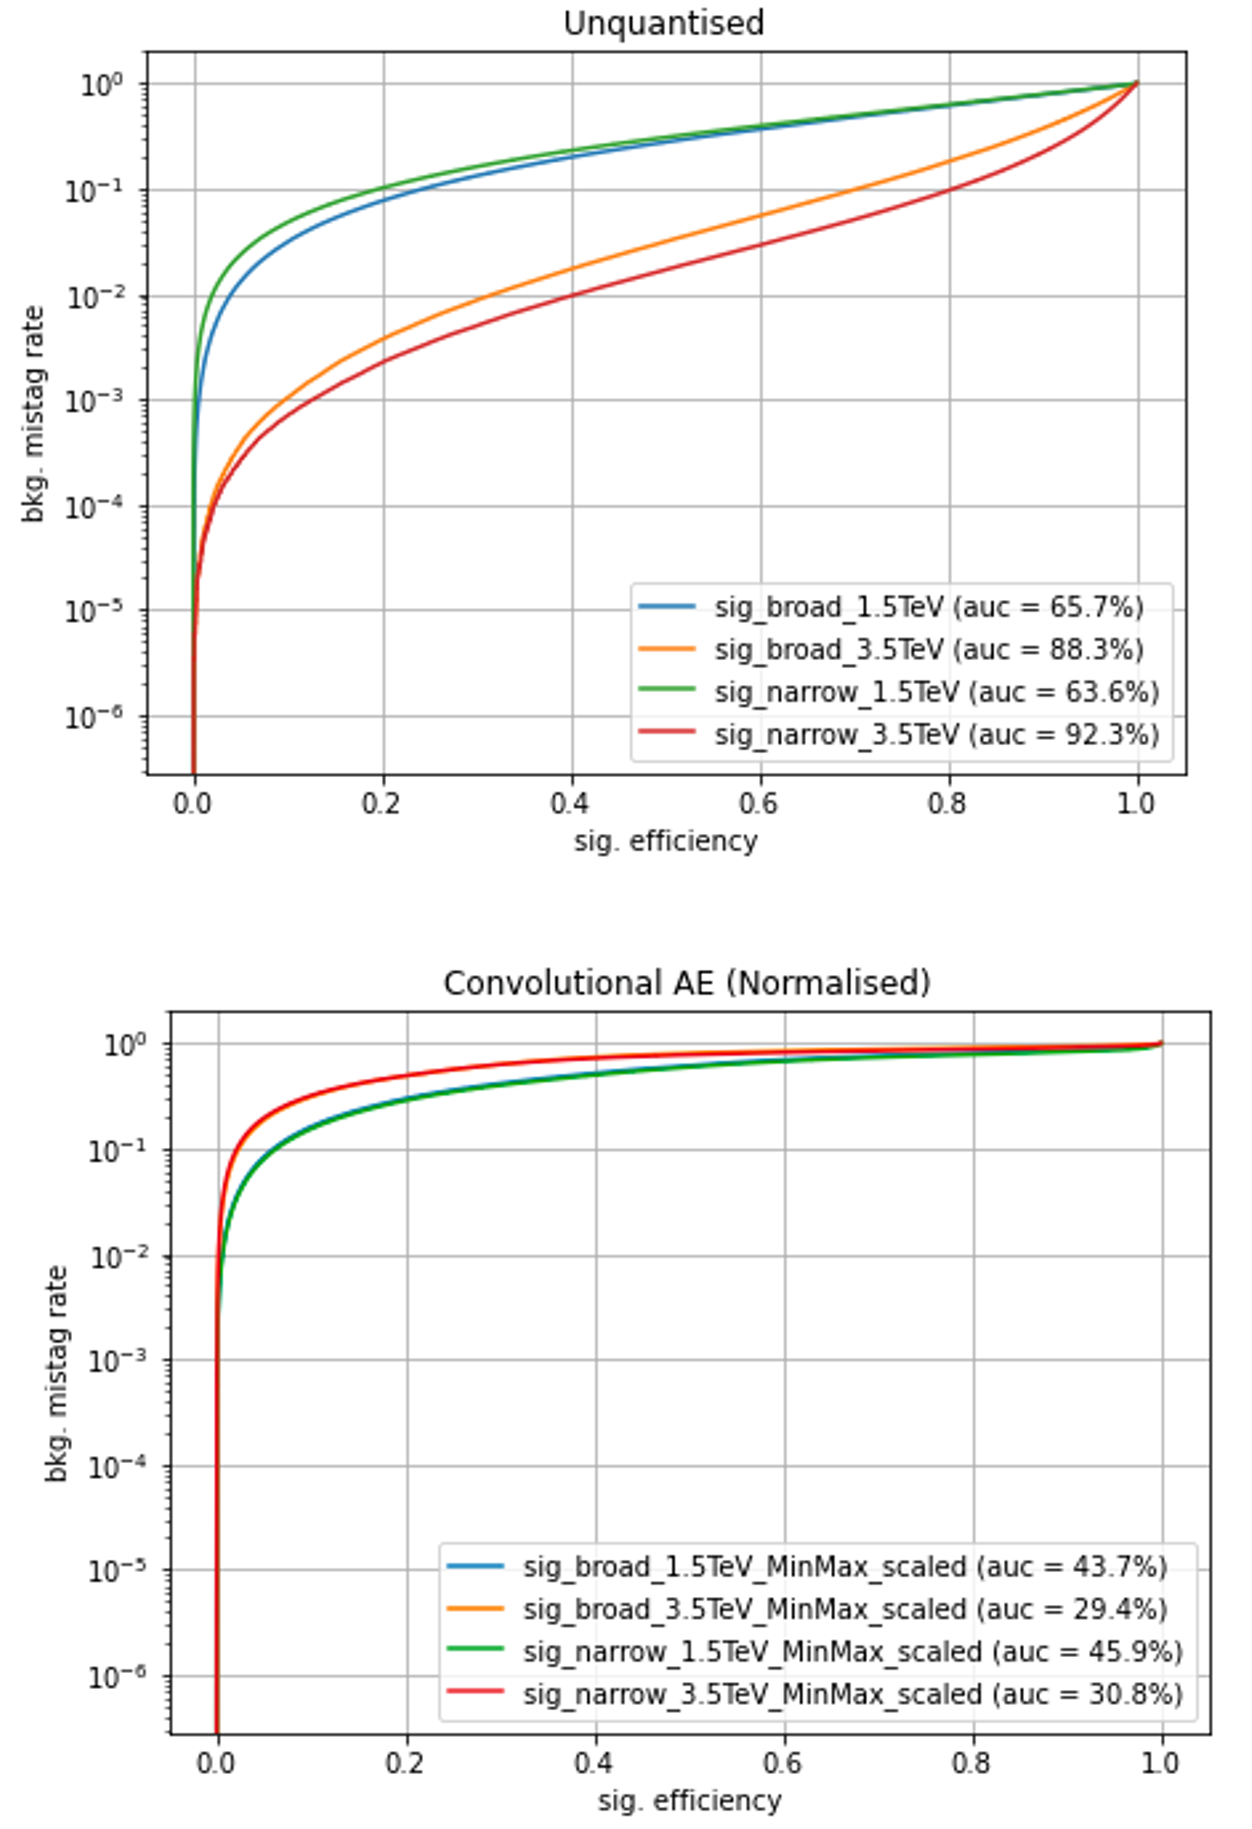
\includegraphics[width=\textwidth]{cnn-roc.png}
						\caption{The Receiver Operating Characteristic (ROC) curves and their corresponding Area Under Curve (AUC) scores for the regular CNN AE (top) and the CNN AE with the normlaised datasets (bottom).}
						\label{fig:cnn-roc}
					\end{minipage}
				\hfill
					\begin{minipage}[c]{0.45\linewidth}
						\centering
						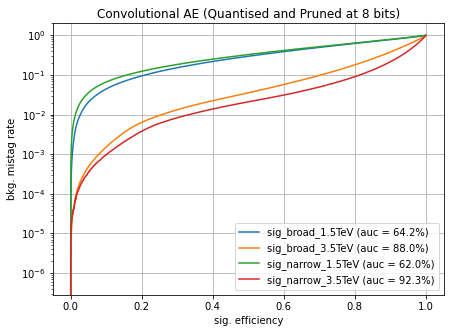
\includegraphics[width=\textwidth]{cnn-compressed-roc.png}
						\caption{he Receiver Operating Characteristic (ROC) curves and their corresponding Area Under Curve (AUC) scores for the quantised and pruned CNN AE model.}
						\label{fig:cnn-compressed-roc}
					\end{minipage}
			\end{figure}

			Shown in Figure \ref{fig:garnet-roc} are the ROC curves and AUC scores for Garnet-Dense on all signal datasets. The model performs poorly when compared to the regular CNN AE AUC scores (Figure \ref{fig:cnn-roc}) - for example - for the $3.5  TeV$ narrow signal dataset, the difference in AUC is a large 33.6\%. This is expected as the training history, feature reconstruction, and loss distribution plots all showed the model not doing as well as expected, and it all comes down to the fact that the model virtually did not train, and so did not fit the data. 

			\begin{figure}[H]
				\centering
				\begin{minipage}[b]{\linewidth}
					\centering
					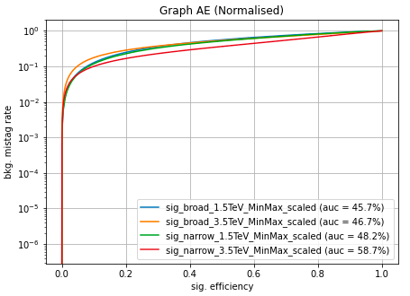
\includegraphics[width=0.5\textwidth]{garnet-roc.png}
					\caption{The Receiver Operating Characteristic (ROC) curves and their corresponding Area Under Curve (AUC) scores for the GarNet-Dense model (normalised datasets).}
					\label{fig:garnet-roc}
				\end{minipage}
			\end{figure}


    \section{Conclusion}
    \label{section:conclusion}

	 To conclude, autoencoders were explored to see how viable they are for new physics anomaly detection for the upcoming High-Luminosity LHC upgrade. Two model architectures were tested - CNN and GarNet-Dense. The CNN model produced good results, with AUC scores as high as 92.3\% for the narrow band $3.5 TeV$ signal dataset, and so it is able to detect anomalies in the signal data; this is especially the case with the signal datasets that have the higher mass value of $3.5 TeV$. The GarNet-Dense on the other hand produces poor results due to the model not being able to train regardless of many efforts employed to make it train (such as normalising the data), so it cannot be recommended to use the GarNet-Dense architecture in the L1T for HL-LHC. It was also shown that normalising the datasets for CNNs, while it removes the data bias, produces overall worse results. Also, quantising the number of bits down to 8-bits from 32-bits and pruning half the number of weights leads to a significant reduction in the CNN model size, and yet most of the performance of the CNN model remains. We can recommend the use of CNNs for anomaly detection at the L1T for the HL-LHC upgrade.
	
	\newpage
	\bibliography{report}
	
	\appendix
	
\end{document}
